%----------------------------------------------------------------------------
\chapter{Monitor generálás terv és feladat megfogalmazása}
%----------------------------------------------------------------------------

\begin{figure}[!ht]
    \centering
    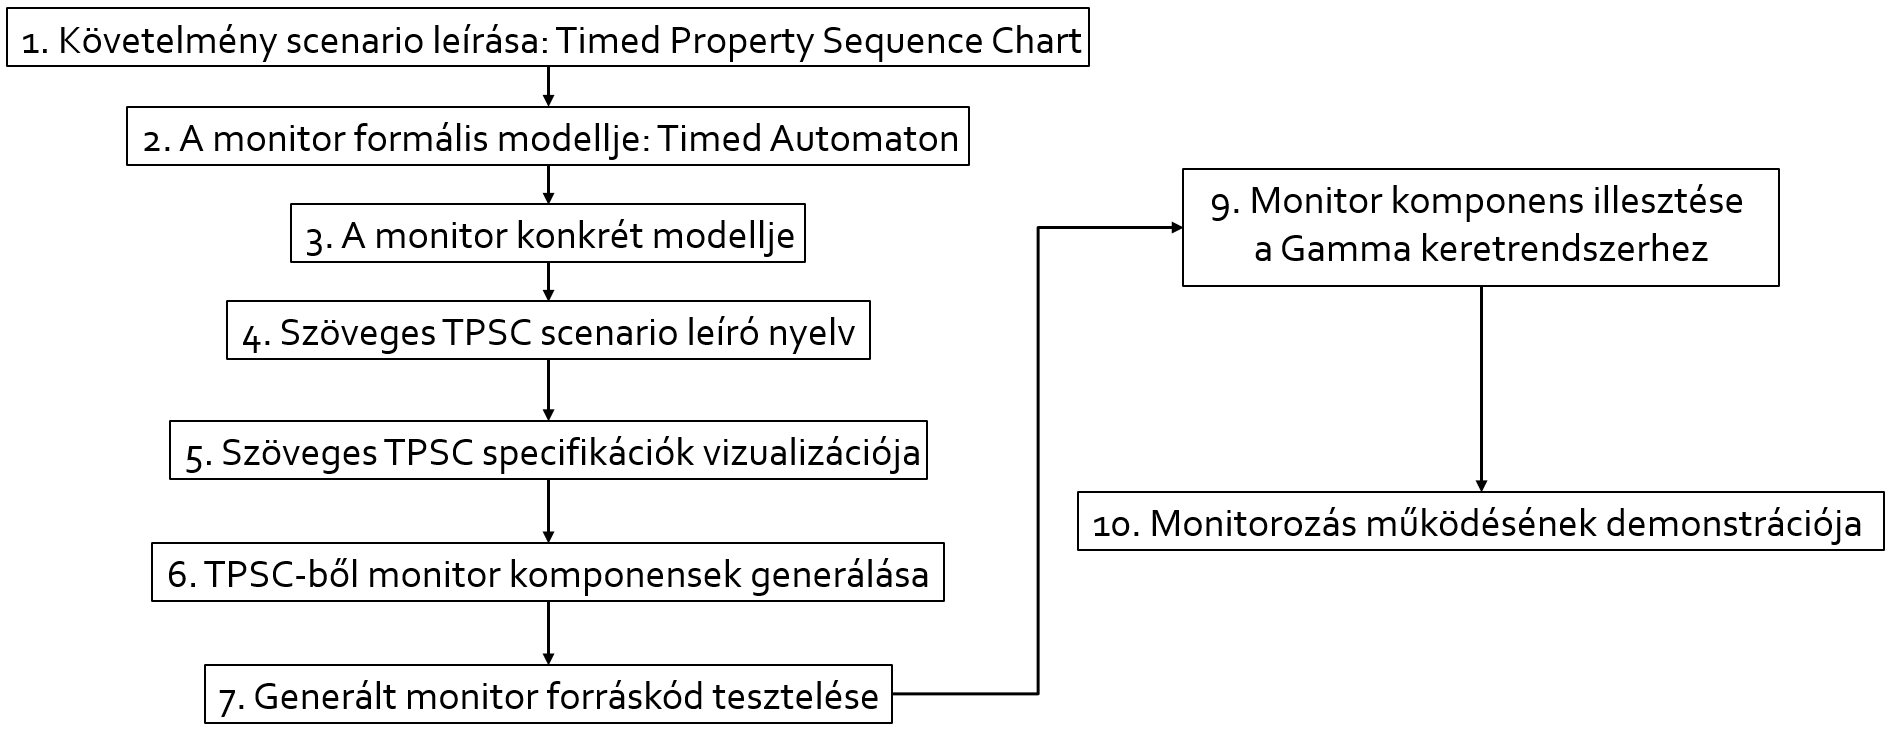
\includegraphics[width=150mm, keepaspectratio]{figures/generation_plan.png}
    \caption{Monitor generátor kibővítése.}
\end{figure}

A cél az, hogy a „Monitor komponensek generálása kontextusfüggő viselkedés ellenőrzése” című szakdolgozatom során elkészített monitor komponens generátort kibővíteni úgy, hogy támogassa időzítési feltételek megadását.
A monitor generálás terve látható a 5.1. ábrán.
Először az a feladatunk, hogy a szakdolgozat során definiált szöveges PSC diagram leíró nyelvet kibővitsük a TPSC elemeivel.
Ezután az automata generátort kell úgy kibővíteni, hogy a TPSC diagramokból tudjon TA automatákat generálni.
Egy monitor forráskód generátor pedig az automata alapján elkészítheti a monitor forráskódját.

A szöveges TPSC scenario leírásához el kell készítenünk a diagram vizualizációját, hogy grafikusan megtekinthessük a definiál scenario-t.
A következő a generált monitor forráskód tesztelése, majd ezután ezt illeszük a Gamma keretrendszerhez.
Ezzel az a célunk, hogy elosztott komponens alapú rendszerek szimulációja közben monitorozható legyen a TPSC üzenet szekvencia specifikáció teljesülése illetve az ebben rögzített tulajdonságok megsértése

A Diplomatervezés 1 tárgy keretében a tervnek a negyedik, hatodik és hetedik részeivel foglalkoztam.